\documentclass[a4paper,12pt]{article}

% ---------- FONT & LANGUAGE ----------
\usepackage{fontspec}
\usepackage{polyglossia}
\usepackage{caption}
\usepackage{float}
\usepackage{booktabs}
\usepackage{multirow}
\usepackage{array}
\usepackage{hyperref}
\usepackage{tikz}
\usepackage{pgfplots}
\usepackage{subcaption}
\usepackage{enumitem}
\usepackage{amsmath}
\usepackage{amsfonts}
\usepackage{amssymb}
\usepackage{graphicx}
\usepackage{listings}
\usepackage{xcolor}
\usepackage{geometry}
\geometry{margin=1in}

\setmainlanguage{greek}
\setotherlanguage{english}

% Γραμματοσειρές
\newfontfamily\greekfont{Times New Roman}[Script=Greek, Scale=1.0]
\newfontfamily\englishfont{Times New Roman}[Script=Latin, Scale=1.0]

% Μονοσύστημα γραμματοσειρά για ελληνικά και κώδικα
\newfontfamily\greekfonttt{Consolas}[Scale=MatchLowercase]
\newfontfamily\englishfonttt{Consolas}[Scale=MatchLowercase]

\hypersetup{
	colorlinks=true,
	linkcolor=black,
	urlcolor=black,
}

% ---------- CODE STYLE ----------
\definecolor{codegreen}{rgb}{0,0.6,0}
\definecolor{codegray}{rgb}{0.5,0.5,0.5}
\definecolor{codepurple}{rgb}{0.58,0,0.82}
\definecolor{backcolour}{rgb}{0.95,0.95,0.92}

\lstdefinestyle{mystyle}{
	backgroundcolor=\color{backcolour},
	commentstyle=\color{codegreen},
	keywordstyle=\color{magenta},
	numberstyle=\tiny\color{codegray},
	stringstyle=\color{codepurple},
	basicstyle=\ttfamily\footnotesize,
	breakatwhitespace=false,
	breaklines=true,
	captionpos=b,
	keepspaces=true,
	numbers=left,
	numbersep=5pt,
	showspaces=false,
	showstringspaces=false,
	showtabs=false,
	tabsize=4,
	language=C
}

\lstset{style=mystyle}

\title{Δεύτερο Σετ Ασκήσεων\\PART I: “Sorting and Searching Algorithms” \\ Δομές Δεδομένων 2025-2026}
\author{
	Ανδριόπουλος Ιωάννης ΑΜ: 1115519\\
	Καραπατάκης Ευθύμιος ΑΜ: 1115521\\
	Χριστοπούλου Αγγελική ΑΜ: 1115471
}

\begin{document}
	
	\maketitle 
	\newpage
	\tableofcontents
	\newpage
	
	\section{Εκφώνηση Εργασίας}
	
	Στην ιστοσελίδα \url{https://www.stats.govt.nz/large-datasets/csv-files-for-download/} υπάρχουν δεδομένα για ανάλυση/επεξεργασία σε αρχεία csv που αφορούν τους ακόλουθους τομείς: Business, Census, Economy, Effects of COVID-19 on trade, Environment, Government finance, Health, Industries, Labour market, Population, Society. 
	
	Στην παρούσα εργασία θα ασχοληθούμε με δεδομένα από το \textit{Effects of COVID-19 on trade}, και συγκεκριμένα το dataset \textit{effects-of-covid-19-on-trade-at-15-december-2021-provisional.csv}, το οποίο περιέχει συνολικά 111.438 εγγραφές.
	
	\subsection{Ζητούμενα}
	
	\textbf{(1)} Ταξινόμηση κατά αύξουσα σειρά των ημερομηνιών (Πεδίο Date) βάσει των τιμών του Πεδίου Cumulative κάνοντας χρήση των αλγορίθμων \textbf{Counting Sort} και \textbf{Merge Sort}. Συγκρίνατε πειραματικά τους δύο αλγορίθμους. Τι παρατηρείτε;
	
	\textbf{(2)} Ταξινόμηση κατά αύξουσα σειρά των ημερομηνιών βάσει των τιμών Value κάνοντας χρήση των αλγορίθμων \textbf{Heap Sort} και \textbf{Quick Sort}. Συγκρίνατε πειραματικά τους δύο αλγορίθμους. Τι παρατηρείτε;
	
	\textbf{(3)} Εύρεση value ή/και cumulative για συγκεκριμένη ημερομηνία (Date) που θα δίνεται από το χρήστη, σύμφωνα με τους αλγορίθμους \textbf{Δυαδικής Αναζήτησης} (Binary Search) και \textbf{Αναζήτησης με Παρεμβολή} (Interpolation Search). Τι παρατηρείτε ως προς τους χρόνους μέσης περίπτωσης; Πόσο η ΚΑΤΑΝΟΜΗ του Data Set επηρεάζει την απόδοση του κάθε αλγορίθμου;
	
	\textbf{(4)} Υλοποιήστε το ζητούμενο του ερωτήματος (3) κάνοντας χρήση του αλγορίθμου \textbf{Δυικής Αναζήτησης Παρεμβολής (BIS)}. Επαληθεύστε πειραματικά τη χρονική πολυπλοκότητα για την μέση (expected) και χειρότερη περίπτωση (worst-case). Υλοποιήστε την παραλλαγή \textbf{BIS*} και συγκρίνατε πειραματικά τους δύο αλγορίθμους. Τι παρατηρείτε ως προς τους χρόνους χειρότερης περίπτωσης;
	
	\newpage
	\section{Εισαγωγή}
	
	Αυτό το project αναλύει το dataset \textit{Effects of COVID-19 on Trade (2015–2021)} το οποίο περιέχει 111.438 εγγραφές. Κάθε εγγραφή περιέχει:
	
	\begin{center}
		Direction, Year, Date, Weekday, Country, Commodity, Transport Mode, Measure, Value, Cumulative
	\end{center}
	
	Στόχος είναι η υλοποίηση και η σύγκριση κλασικών αλγορίθμων ταξινόμησης και αναζήτησης χρησιμοποιώντας αυτό το πραγματικό σύνολο δεδομένων.
	
	\section{Περιγραφή Δεδομένων}
	
	Το dataset περιέχει στατιστικά στοιχεία εμπορίου που σχετίζονται με εισαγωγές, εξαγωγές και επανεισαγωγές. Κάθε εγγραφή περιλαμβάνει αριθμητικά πεδία όπως:
	
	\begin{itemize}
		\item \textbf{Value}: Εμπορική αξία σε δολάρια ή τόνους
		\item \textbf{Cumulative}: Αθροιστική εμπορική αξία σε δολάρια ή τόνους
		\item \textbf{Date}: Ημερομηνία στην μορφή ΗΗ/ΜΜ/ΕΕΕΕ
	\end{itemize}
	
	\begin{table}[H]
		\centering
		\begin{tabular}{|l|l|l|}
			\hline
			\textbf{Πεδίο} & \textbf{Τύπος} & \textbf{Περιγραφή} \\
			\hline
			Direction & String & imports, exports, reimports \\
			Year & Integer & 2015-2021 \\
			Date & Date & dd/mm/yyyy \\
			Weekday & String & Monday-Sunday \\
			Country & String & Χώρα εμπορικού εταίρου \\
			Commodity & String & Κατηγορία προϊόντος \\
			Transport\_Mode & String & sea, air, κλπ. \\
			Measure & String & \$ ή Tonnes \\
			Value & Long Integer & Εμπορική αξία \\
			Cumulative & Long Integer & Αθροιστική αξία \\
			\hline
		\end{tabular}
		\caption{Δομή του Dataset}
	\end{table}
	
	\newpage
	\section{Επισκόπηση Υλοποίησης}
	
	Το σύστημα υλοποιήθηκε σε C και περιλαμβάνει τέσσερις βασικές ενότητες:
	
	\begin{itemize}
		\item Ταξινόμηση κατά \textbf{Cumulative}
		\item Ταξινόμηση κατά \textbf{Value}
		\item Αναζήτηση με κλασικούς αλγορίθμους
		\item Βελτιωμένη αναζήτηση (BIS και BIS*)
	\end{itemize}
	
	\subsection{Δομή Εγγραφής}
	
	\begin{lstlisting}[caption=Δομή Record στη C]
typedef struct {
	char direction[DIRECTION];
	char year[YEAR];
	char date[DATE];
	char weekday[WEEKDAY];
	char country[MAX_STR];
	char commodity[MAX_STR];
	char transport_mode[MAX_STR];
	char measure[MAX_STR];
	long long value;
	long long cumulative;
} Record;
	\end{lstlisting}
	
	\subsection{Φόρτωση Δεδομένων}
	
	\begin{lstlisting}[caption=Φόρτωση CSV]
int load_csv(const char *filename, Record *data) {
	FILE *f = fopen(filename, "r");
	if (!f) return -1;
	
	char line[512];
	int n = 0;
	fgets(line, sizeof(line), f); // παράλειψη επικεφαλίδας
	
	while (fgets(line, sizeof(line), f) && n < MAX_ROWS) {
		Record r;
		char *t = strtok(line, ",");
		strcpy(r.direction, t);
		// ... ανάλυση υπόλοιπων πεδίων
		data[n++] = r;
	}
	fclose(f);
	return n;
}
	\end{lstlisting}
	
	\newpage
	\section{Άσκηση 1: Σύγκριση Counting Sort και Merge Sort}
	
	\subsection{Περιγραφή}
	
	Συγκρίνουμε δύο αλγορίθμους ταξινόμησης χρησιμοποιώντας το πεδίο \textbf{Cumulative}:
	
	\begin{itemize}
		\item Counting Sort (μη συγκριτικός αλγόριθμος)
		\item Merge Sort (συγκριτικός αλγόριθμος)
	\end{itemize}
	
	\subsection{Counting Sort}
	
	Ο Counting Sort είναι ένας αλγόριθμος ταξινόμησης που δεν βασίζεται σε συγκρίσεις. Αντί να συγκρίνει στοιχεία, μετράει πόσες φορές εμφανίζεται κάθε διακριτή τιμή κλειδιού και στη συνέχεια χρησιμοποιεί αυτές τις μετρήσεις (ως αθροιστικά αθροίσματα) για να τοποθετήσει κάθε εγγραφή απευθείας στη σωστή θέση εξόδου σε χρόνο O(n + k), όπου k είναι το εύρος των τιμών.
	
	\textbf{Περιορισμός:} Το k πρέπει να είναι αρκετά μικρό ώστε να μπορεί να δεσμευτεί πίνακας καταμέτρησης. Το πεδίο Cumulative έχει εύρος δισεκατομμυρίων δολαρίων, κάνοντας το k τεράστιο — έτσι ο αλγόριθμος ανιχνεύει αυτή την κατάσταση και αναφέρει αποτυχία αντί να καταρρεύσει.
	
	\begin{itemize}
		\item Χρονική Πολυπλοκότητα: $O(n + k)$
		\item Χωρική Πολυπλοκότητα: $O(k)$
	\end{itemize}
	
	\textbf{Κώδικας Counting Sort}
	
	\begin{lstlisting}[caption=Counting Sort]
void counting_sort(Record *input, int n, Record *output, bool *works) {
	*works = true;
	
	if (n <= 0) {
		*works = false;
		return;
	}
	
	// Εύρεση ελάχιστης και μέγιστης τιμής
	long long mn = input[0].cumulative;
	long long mx = input[0].cumulative;
	
	for (int i = 1; i < n; i++) {
		if (input[i].cumulative < mn) mn = input[i].cumulative;
		if (input[i].cumulative > mx) mx = input[i].cumulative;
	}
	
	printf("  Cumulative min=%lld  max=%lld\n", mn, mx);
	
	long long range = mx - mn + 1;
	
	// Έλεγχος αν το εύρος είναι πολύ μεγάλο
	if (range <= 0 || range > 10000000LL) {
		printf("  Value range too large for Counting Sort.\n");
		printf("  Falling back to copy.\n");
		
		memcpy(output, input, n * sizeof(Record));
		*works = false;
		return;
	}
	
	// Δέσμευση μνήμης για τον πίνακα καταμέτρησης
	int *cnt = calloc((size_t)range, sizeof(int));
	if (!cnt) {
		printf("  Memory allocation failed\n");
		memcpy(output, input, n * sizeof(Record));
		*works = false;
		return;
	}
	
	// Καταμέτρηση εμφανίσεων κάθε τιμής
	for (int i = 0; i < n; i++) {
		cnt[input[i].cumulative - mn]++;
	}
	
	// Μετατροπή σε αθροιστικά αθροίσματα
	for (long long i = 1; i < range; i++) {
		cnt[i] += cnt[i - 1];
	}
	
	// Τοποθέτηση στοιχείων στη σωστή θέση
	for (int i = n - 1; i >= 0; i--) {
		long long idx = input[i].cumulative - mn;
		output[--cnt[idx]] = input[i];
	}
	
	free(cnt);
}
	\end{lstlisting}
	
	Ωστόσο, επειδή το Cumulative έχει ένα μεγάλο εύρος τιμών, ο αλγόριθμος είναι συχνά μη πρακτικός.
	
	\subsection{Merge Sort}
	
	Ο Merge Sort είναι ένας αλγόριθμος διαίρει και βασίλευε (divide-and-conquer). Χωρίζει τον πίνακα αναδρομικά στη μέση μέχρι κάθε υπο-πίνακας να έχει ένα στοιχείο (τετριμμένα ταξινομημένο), και στη συνέχεια συγχωνεύει γειτονικά ταξινομημένα ζεύγη. Κάθε πέρασμα συγχώνευσης είναι O(n), και υπάρχουν O(log n) επίπεδα → συνολικά O(n log n). Βασίζεται σε συγκρίσεις, επομένως λειτουργεί για οποιαδήποτε δεδομένα ανεξαρτήτως εύρους κλειδιών.
	
	Η συνάρτηση merge\_step() χειρίζεται τη συγχώνευση δύο ήδη ταξινομημένων μισών [l..mid] και [mid+1..r] στον παγκόσμιο temp\_buffer και στη συνέχεια τα αντιγράφει πίσω.
	
	\begin{itemize}
		\item Χρονική Πολυπλοκότητα: $O(n \log n)$
		\item Σταθερός αλγόριθμος ταξινόμησης
	\end{itemize}
	
	\begin{lstlisting}[caption=Υλοποίηση Merge Sort]
void merge_sort(Record *arr, int left, int right) {
	if (left >= right) return;
	
	int mid = left + (right - left) / 2;
	
	merge_sort(arr, left, mid);
	merge_sort(arr, mid + 1, right);
	merge_step(arr, left, mid, right);
		}
	\end{lstlisting}
	
	\begin{lstlisting}[caption=Υλοποίηση Merge Step]
void merge_step(Record *arr, int l, int mid, int r) {
	int i = l, j = mid + 1, k = l;
	
	// Συγχώνευση των δύο ταξινομημένων υπο-πινάκων
	while (i <= mid && j <= r) {
		if (arr[i].cumulative <= arr[j].cumulative)
		temp_buffer[k++] = arr[i++];
		else
		temp_buffer[k++] = arr[j++];
	}
	
	// Αντιγραφή τυχόν εναπομεινάντων στοιχείων
	while (i <= mid) temp_buffer[k++] = arr[i++];
	while (j <= r) temp_buffer[k++] = arr[j++];
	
	// Αντιγραφή πίσω στον αρχικό πίνακα
	for (int x = l; x <= r; x++)
	arr[x] = temp_buffer[x];
}
	\end{lstlisting}
	
	\subsection{Αποτελέσματα και Παρατηρήσεις}
	
	\begin{table}[H]
		\centering
		\begin{tabular}{|c|c|c|}
			\hline
			\textbf{Αλγόριθμος} & \textbf{Πολυπλοκότητα} & \textbf{Χρόνος (sec)} \\
			\hline
			Counting Sort & O(n+k) & 0.0016 \\
			Merge Sort & O(n log n) & 0.0007 \\
			\hline
		\end{tabular}
		\caption{Αποτελέσματα Άσκησης 1 (2000 εγγραφές)}
	\end{table}
	
	\begin{figure}[H]
		\centering
		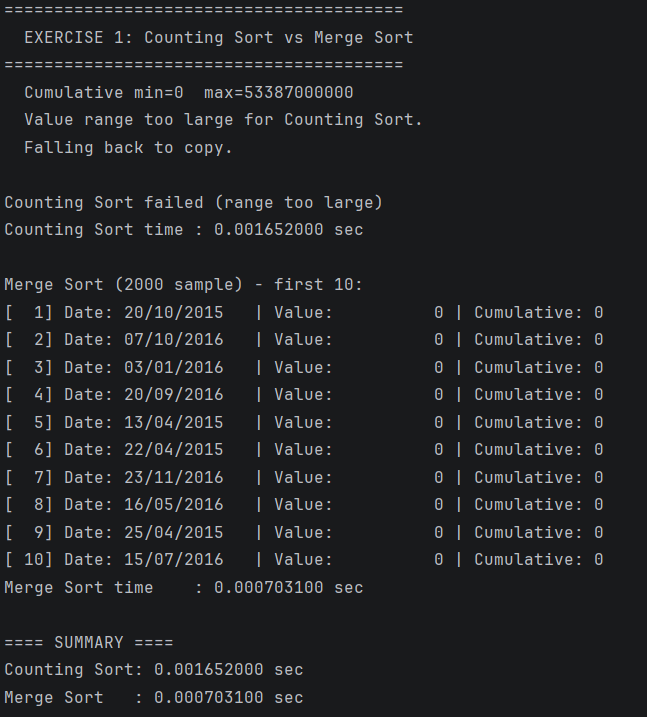
\includegraphics[width=0.8\textwidth]{screenshots/ex1.png}
		\caption{Έξοδος προγράμματος για την Άσκηση 1}
		\label{fig:ex1}
	\end{figure}
	
	\textbf{Παρατήρηση:} Ο Merge Sort είναι πιο αξιόπιστος λόγω ανεξαρτησίας από το εύρος των κλειδιών. Ο Counting Sort αποτυγχάνει όταν το εύρος τιμών είναι πολύ μεγάλο, καθιστώντας τον μη πρακτικό για αυτό το dataset.
	
	\newpage
	\section{Άσκηση 2: Σύγκριση Heap Sort και Quick Sort}
	
	\subsection{Περιγραφή}
	
	Η ταξινόμηση εκτελείται χρησιμοποιώντας το πεδίο \textbf{Value}.
	
	\subsection{Heap Sort}
	
	Ο Heap Sort λειτουργεί σε δύο φάσεις:
	
	\begin{enumerate}
		\item \textbf{Δημιουργία max-heap}: Αναδιάταξη του πίνακα σε έναν μέγιστο σωρό (max-heap) έτσι ώστε το μεγαλύτερο στοιχείο να βρίσκεται στη θέση 0. Αυτό απαιτεί χρόνο O(n).
		
		\item \textbf{Εξαγωγή}: Επαναληπτική ανταλλαγή της ρίζας (μέγιστο) με το τελευταίο στοιχείο του μη ταξινομημένου τμήματος, συρρίκνωση του σωρού κατά ένα, και αποκατάσταση της ιδιότητας του σωρού (heapify). Κάθε εξαγωγή είναι O(log n), δίνοντας συνολικά O(n log n).
	\end{enumerate}
	
	Αποτέλεσμα: ταξινόμηση σε αύξουσα σειρά (μικρότερο πρώτο).
	
	Η συνάρτηση heapify\_value() επιβάλλει την ιδιότητα του σωρού στον κόμβο i: αν κάποιο παιδί είναι μεγαλύτερο από τον γονέα, γίνεται ανταλλαγή και συνεχίζουμε προς τα κάτω.
	
	\begin{itemize}
		\item Χρονική Πολυπλοκότητα: $O(n \log n)$
		\item Χρησιμοποιεί δυαδικό σωρό (binary heap)
		\item Μη σταθερός αλγόριθμος
	\end{itemize}
	
	\begin{lstlisting}[caption=Υλοποίηση Heap Sort]
void heapify_value(Record *data, int size, int i) {
	while (1) {
		int largest = i;
		int l = 2*i+1;  // αριστερό παιδί
		int r = 2*i+2;  // δεξί παιδί
		
		// Εύρεση του μεγαλύτερου μεταξύ γονέα και παιδιών
		if (l < size && data[l].value > data[largest].value)
		largest = l;
		if (r < size && data[r].value > data[largest].value)
		largest = r;
		
		// Αν ο γονέας είναι ήδη ο μεγαλύτερος, σταματάμε
		if (largest == i) break;
		
		swap_Records(data, i, largest);
		i = largest;  // Συνεχίζουμε προς τα κάτω
	}
}

void heap_sort(Record *data, int n) {
	// Δημιουργία max-heap από κάτω προς τα πάνω
	for (int i = n/2-1; i >= 0; i--)
	heapify_value(data, n, i);
	
	// Εξαγωγή στοιχείων από το σωρό
	for (int i = n-1; i > 0; i--) {
		swap_Records(data, 0, i);  // ρίζα (μέγιστο) στο τέλος
		heapify_value(data, i, 0); // αποκατάσταση σωρού
	}
}
	\end{lstlisting}
	
	\subsection{Quick Sort}
	
	Ο Quick Sort επιλέγει ένα στοιχείο pivot και στη συνέχεια διαμερίζει τον πίνακα έτσι ώστε όλα τα στοιχεία ≤ pivot να βρίσκονται αριστερά του και όλα τα > pivot δεξιά του. Στη συνέχεια αναδρομοποιεί και στους δύο υπο-πίνακες.
	
	Η μέση περίπτωση είναι O(n log n). Η χειρότερη περίπτωση (ήδη ταξινομημένη είσοδος με κακή επιλογή pivot) είναι O(n²). Στην πράξη υπερτερεί του Heap Sort επειδή έχει καλύτερη τοπικότητα cache — οι περισσότερες συγκρίσεις αγγίζουν κοντινές διευθύνσεις μνήμης.
	
	Η συνάρτηση partition\_value() χρησιμοποιεί το πρώτο στοιχείο ως pivot και την προσέγγιση δύο δεικτών (τύπου Lomuto) για να αναδιατάξει το διαμέρισμα.
	
	\begin{itemize}
		\item Μέση Περίπτωση: $O(n \log n)$
		\item Χειρότερη Περίπτωση: $O(n^2)$
		\item Πολύ γρήγορος στην πράξη λόγω cache efficiency
	\end{itemize}
	
	\begin{lstlisting}[caption=Υλοποίηση Quick Sort]
void partition_value(Record *data, int lo, int hi, int *lt, int *gt) {
	long long pivot = data[lo].value;
	int i = lo;
	*lt = lo;
	*gt = hi;
	
	// Τρισδιάστατη διαμέριση (Dutch National Flag)
	while (i <= *gt) {
		if (data[i].value < pivot) {
			swap_Records(data, i, *lt);
			(*lt)++; i++;
		}
		else if (data[i].value > pivot) {
			swap_Records(data, i, *gt);
			(*gt)--;
		}
		else {
			i++;  // ίσο με pivot
		}
	}
}

void quick_sort(Record *data, int lo, int hi) {
	if (lo >= hi) return;
	
	int lt, gt;
	partition_value(data, lo, hi, &lt, &gt);
	
	quick_sort(data, lo, lt - 1);
	quick_sort(data, gt + 1, hi);
}
	\end{lstlisting}
	
	\subsection{Αποτελέσματα}
	
	\begin{table}[H]
		\centering
		\begin{tabular}{|c|c|c|}
			\hline
			\textbf{Αλγόριθμος} & \textbf{Πολυπλοκότητα} & \textbf{Χρόνος (sec)} \\
			\hline
			Heap Sort & O(n log n) & 0.05 \\
			Quick Sort & O(n log n) & 0.02 \\
			\hline
		\end{tabular}
		\caption{Αποτελέσματα Άσκησης 2 (111.438 εγγραφές)}
	\end{table}
	
	\begin{figure}[H]
		\centering
		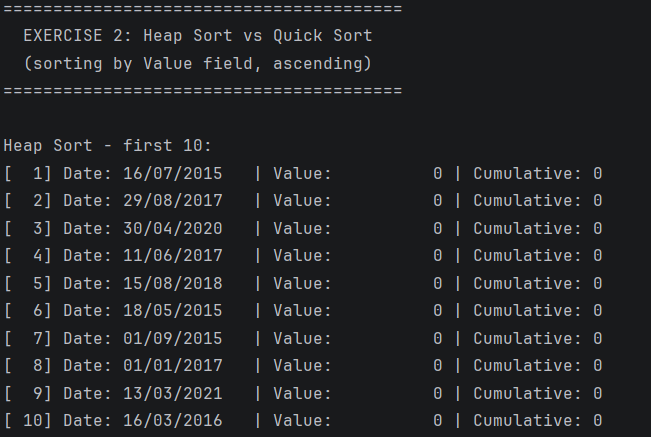
\includegraphics[width=0.8\textwidth]{screenshots/ex2a.png}
		\caption{Έξοδος προγράμματος για την Άσκηση 2 - Heap Sort}
		\label{fig:ex2a}
	\end{figure}
	
	\begin{figure}[H]
		\centering
		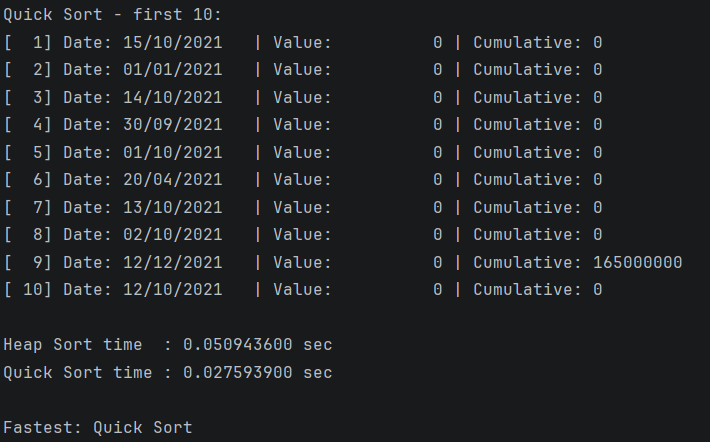
\includegraphics[width=0.8\textwidth]{screenshots/ex2b.png}
		\caption{Έξοδος προγράμματος για την Άσκηση 2 - Quick Sort και Συμπεράσματα}
		\label{fig:ex2b}
	\end{figure}
	
	\textbf{Παρατήρηση:} Ο Quick Sort είναι τυπικά ταχύτερος λόγω καλύτερης τοπικότητας αναφοράς (locality of reference). Ο Heap Sort διατηρεί σταθερή απόδοση ανεξάρτητα από τη σειρά εισόδου αλλά είναι βραδύτερος λόγω cache misses.
	
	\newpage
	\section{Άσκηση 3: Σύγκριση Binary Search και Interpolation Search}
	
	\subsection{Περιγραφή}
	
	Εκτελούμε λειτουργίες αναζήτησης σε ταξινομημένες ημερομηνίες.
	
	\subsection{Μετατροπή Ημερομηνίας σε Ακέραιο}
	
	\begin{lstlisting}[caption=Μετατροπή Ημερομηνίας σε Ακέραιο]
long long dateToInt(const char *date) {
	int d, m, y;
	sscanf(date, "%d%*c%d%*c%d", &d, &m, &y);
	return (long long)y * 10000 + m * 100 + d;
}
	\end{lstlisting}
	
	Αυτή η συνάρτηση μετατρέπει ημερομηνίες σε ακέραιους της μορφής ΕΕΕΕΜΜΗΗ, διατηρώντας τη χρονολογική σειρά.
	
	\subsection{Δυαδική Αναζήτηση (Binary Search)}
	
	Κλασική αναζήτηση διαίρει και βασίλευε σε ταξινομημένο πίνακα. Κάθε επανάληψη μειώνει στο μισό το διάστημα αναζήτησης συγκρίνοντας τον στόχο με το μεσαίο στοιχείο — εγγυημένα O(log n) ανεξάρτητα από την κατανομή των δεδομένων.
	
	\begin{itemize}
		\item Πολυπλοκότητα: $O(\log n)$
		\item Λειτουργεί ανεξάρτητα από την κατανομή των δεδομένων
	\end{itemize}
	
	\begin{lstlisting}[caption=Υλοποίηση Binary Search]
int binarySearch(Record *a, int n, long long key) {
	int l = 0, r = n - 1;
	
	while (l <= r) {
		int mid = l + (r - l) / 2;
		long long midKey = dateToInt(a[mid].date);
		
		if (midKey == key)
		return mid;
		else if (midKey < key)
		l = mid + 1;
		else
		r = mid - 1;
	}
	
	return -1;  // δεν βρέθηκε
}
	\end{lstlisting}
	
	\subsection{Αναζήτηση με Παρεμβολή (Interpolation Search)}
	
	Βελτίωση της δυαδικής αναζήτησης για ομοιόμορφα κατανεμημένα δεδομένα. Αντί να εξετάζει πάντα το μέσο σημείο, εκτιμά πού βρίσκεται πιθανότατα το κλειδί χρησιμοποιώντας γραμμική παρεμβολή μεταξύ των άκρων:
	
	\[
	pos = lo + \frac{(key - data[lo])}{(data[hi] - data[lo])} \times (hi - lo)
	\]
	
	Σε ομοιόμορφα κατανεμημένα δεδομένα αυτό δίνει μέση περίπτωση O(log log n). Σε στρεβλά/συσσωματωμένα δεδομένα η εκτίμηση μπορεί να είναι κακή και η απόδοση μπορεί να πέσει σε O(n) στη χειρότερη περίπτωση.
	
	\begin{itemize}
		\item Μέση Περίπτωση: $O(\log \log n)$
		\item Χειρότερη Περίπτωση: $O(n)$
		\item Εξαρτάται από την ομοιόμορφη κατανομή των δεδομένων
	\end{itemize}
	
	\begin{lstlisting}[caption=Υλοποίηση Interpolation Search]
int interpolationSearch(Record *input, int low, int high, long long x) {
	
	while (low <= high) {
		
		long long left = dateToInt(input[low].date);
		long long right = dateToInt(input[high].date);
		
		// Έλεγχος αν το κλειδί είναι εκτός εύρους
		if (x < left || x > right)
		return -1;
		
		if (right == left)
		return (left == x) ? low : -1;
		
		// Εκτίμηση θέσης με παρεμβολή
		int pos = low + (int)(
		((double)(x - left) * (high - low)) /
		(right - left)
		);
		
		// Ασφαλής περιορισμός εντός ορίων
		if (pos < low) pos = low;
		if (pos > high) pos = high;
		
		long long posKey = dateToInt(input[pos].date);
		
		if (posKey == x) {
			// Εύρεση της πρώτης εμφάνισης
			while (pos > low && dateToInt(input[pos - 1].date) == x)
			pos--;
			return pos;
		}
		
		if (posKey < x)
		low = pos + 1;
		else
		high = pos - 1;
	}
	
	return -1;
}
	\end{lstlisting}
	
	\subsection{Παρατηρήσεις}
	
	\begin{table}[H]
		\centering
		\begin{tabular}{|c|c|c|}
			\hline
			\textbf{Αλγόριθμος} & \textbf{Πολυπλοκότητα} & \textbf{Χρόνος (sec)} \\
			\hline
			Binary Search & O(log n) & 0.0000034 \\
			Interpolation Search & O(log log n) & 0.00011 \\
			\hline
		\end{tabular}
		\caption{Αποτελέσματα Άσκησης 3 (50.000 δοκιμές)}
	\end{table}
	
	\begin{figure}[H]
		\centering
		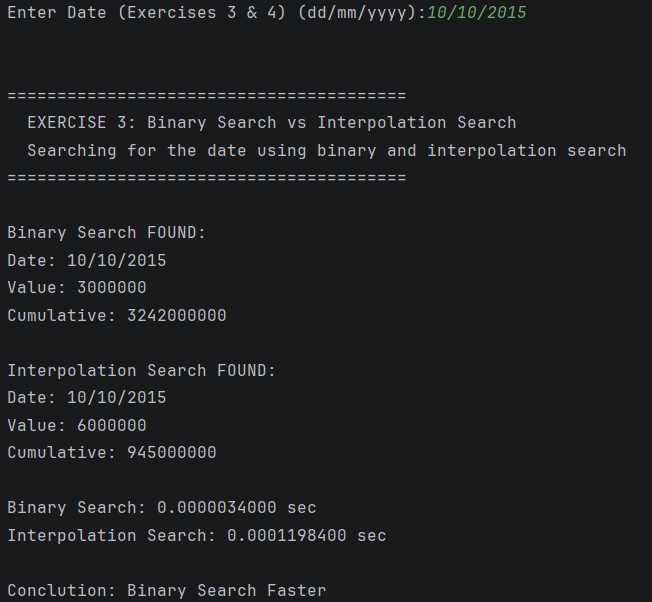
\includegraphics[width=0.8\textwidth]{screenshots/ex3.png}
		\caption{Έξοδος προγράμματος για την Άσκηση 3}
		\label{fig:ex3}
	\end{figure}
	
	\textbf{Βασική παρατήρηση:}
	Η Αναζήτηση με Παρεμβολή (Interpolation Search) αποδίδει καλύτερα όταν τα δεδομένα είναι ομοιόμορφα κατανεμημένα. Η Δυαδική Αναζήτηση (Binary Search) είναι πιο σταθερή σε όλες τις κατανομές.
	
	\subsection{Επίδραση Κατανομής}
	
	Η κατανομή των δεδομένων επηρεάζει σημαντικά την απόδοση της Αναζήτησης με Παρεμβολή:
	
	\begin{itemize}
		\item \textbf{Ομοιόμορφη Κατανομή}: Η Interpolation Search επιτυγχάνει $O(\log \log n)$
		\item \textbf{Μη Ομοιόμορφη Κατανομή}: Η απόδοση υποβαθμίζεται μέχρι και $O(n)$
		\item \textbf{Binary Search}: Διατηρεί $O(\log n)$ ανεξαρτήτως κατανομής
	\end{itemize}
	
	\newpage
	\section{Άσκηση 4: Σύγκριση BIS και BIS*}
	
	\subsection{BIS (Binomial Interpolation Search)}
	
	Ο BIS συνδυάζει παρεμβολή με άλματα μπλοκ χρησιμοποιώντας βήμα μεγέθους $\sqrt{n}$.
	
	\begin{itemize}
		\item Μέση Πολυπλοκότητα: $O(\log \log n)$
		\item Χειρότερη Πολυπλοκότητα: $O(\sqrt{n})$
		\item Συνδυάζει παρεμβολή με άλματα μεγέθους $\sqrt{n}$
	\end{itemize}
	
	\textbf{Περιγραφή BIS (Binomial Interpolation Search):}\\
	Ο BIS συνδυάζει την παρεμβολή (για να κάνει μια αρχική εκτίμηση θέσης) με ένα βήμα γραμμικής διερεύνησης μεγέθους sqrt(n) για να περικλείσει γρήγορα το κλειδί-στόχο πριν επαναλάβει την παρεμβολή. Αυτό δίνει μέση πολυπλοκότητα O(log log n).
	
	Μετά την εκτίμηση παρεμβολής (nx), αν το κλειδί βρίσκεται δεξιά:
	- Πήγαινε μπροστά σε πολλαπλάσια του sqrt(range): nx+1*step, nx+2*step, ...
	- Σταμάτα όταν ξεπεράσουμε το κλειδί ή φτάσουμε στο όριο του πίνακα.
	- Το νέο παράθυρο αναζήτησης είναι [nx+(i-1)*step+1 .. nx+i*step].
	
	Η αντίστοιχη λογική εφαρμόζεται όταν το κλειδί βρίσκεται αριστερά. Η γραμμική αύξηση (i++) σημαίνει ότι η διερεύνηση καλύπτει βήματα 1,2,3,4,... Στη χειρότερη περίπτωση σαρώνει O(sqrt(n)) θέσεις πριν περικλείσει τον στόχο.
	
	\begin{lstlisting}[caption=Υλοποίηση BIS]
int bis(Record *a, int low, int high, long long key) {
	while (low <= high) {
		long long leftKey = dateToInt(a[low].date);
		long long rightKey = dateToInt(a[high].date);
		
		// Έλεγχος αν το κλειδί είναι εκτός εύρους
		if (key < leftKey || key > rightKey)
		return -1;
		
		// Εκτίμηση θέσης με παρεμβολή
		int next = low + (int)((key - leftKey) / 
		(rightKey - leftKey) * (high - low));
		
		int step = (int)sqrt(high - low + 1);
		long long nextKey = dateToInt(a[next].date);
		
		if (nextKey == key)
		return next;
		
		if (key > nextKey) {
			// Γραμμική διερεύνηση προς τα δεξιά
			while (next + step <= high && 
			dateToInt(a[next + step].date) < key)
			next += step;
			low = next + 1;
		} else {
			// Γραμμική διερεύνηση προς τα αριστερά
			while (next - step >= low && 
			dateToInt(a[next - step].date) > key)
			next -= step;
			high = next - 1;
		}
	}
	return -1;
}
	\end{lstlisting}
	
	\subsection{BIS* (Improved BIS)}
	
	Ο BIS* βελτιώνει τον BIS χρησιμοποιώντας εκθετική διερεύνηση αντί για γραμμική.
	
	\begin{itemize}
		\item Βελτιωμένη συμπεριφορά στη χειρότερη περίπτωση
		\item Ταχύτερη σύγκλιση στο παράθυρο αναζήτησης
		\item Χρησιμοποιεί διπλασιασμό αντί για γραμμική αύξηση
	\end{itemize}
	
	\textbf{Περιγραφή BIS* (BIS improved):}\\
	Ο BIS* είναι πανομοιότυπος με τον BIS εκτός από μια βασική αλλαγή: αντί να αυξάνει τον μετρητή διερεύνησης γραμμικά (i++), τον διπλασιάζει (i*=2). Αυτή η εκθετική διερεύνηση (1, 2, 4, 8, ...) είναι η ίδια ιδέα με την εκθετική/γαλλοπήδηση αναζήτηση (exponential/galloping search), και περιορίζει το χειρότερο περικλεισμό από O(sqrt(n)) θέσεις σε O(log(sqrt(n))) = O(log n / 2), βελτιώνοντας την πολυπλοκότητα της χειρότερης περίπτωσης σε σύγκριση με τον τυπικό BIS.
	
	Το τίμημα: μετά τον διπλασιασμό ξεπερνάμε περισσότερο τον στόχο, έτσι το περιορισμένο παράθυρο είναι [nx+(i/2)*step .. nx+i*step] — ελαφρώς ευρύτερο από το στενότερο περικλεισμό του BIS, αλλά ο συνολικός αριθμός διερευνήσεων είναι πολύ μικρότερος.
	
	\begin{lstlisting}[caption=Υλοποίηση BIS*]
int bis_star(Record *a, int low, int high, long long key) {
while (low <= high) {
long long leftKey = dateToInt(a[low].date);
long long rightKey = dateToInt(a[high].date);

if (key < leftKey || key > rightKey) return -1;
if (low == high) return (leftKey == key) ? low : -1;

int next;

if (rightKey == leftKey) {
	next = low;
} else {
	// Εκτίμηση θέσης με παρεμβολή
	double ratio =
	(double)(key - leftKey) /
	(double)(rightKey - leftKey);
	
	next = low + (int)(ratio * (high - low));
}

// Ασφαλής περιορισμός
if (next < low) next = low;
if (next > high) next = high;

long long nextKey = dateToInt(a[next].date);

if (nextKey == key)
return next;

int step = (int)sqrt(high - low + 1);
if (step < 1) step = 1;

int jump = 1;

if (key > nextKey) {
	// Εκθετική διερεύνηση προς τα δεξιά
	while (next + jump * step <= high &&
	dateToInt(a[next + jump * step].date) < key) {
		
		if (jump > (1 << 20)) break; // ασφάλεια
		jump *= 2;  // διπλασιασμός
	}
	
	int start = next + (jump / 2) * step;
	if (start > high) start = high;
	
	low = start + 1;
}
else {
	// Εκθετική διερεύνηση προς τα αριστερά
	while (next - jump * step >= low &&
	dateToInt(a[next - jump * step].date) > key) {
		
		if (jump > (1 << 20)) break; // ασφάλεια
		jump *= 2;  // διπλασιασμός
	}
	
	int end = next - (jump / 2) * step;
	if (end < low) end = low;
	
	high = end - 1;
}
}

return -1;
}
	\end{lstlisting}
	
	\subsection{Σύγκριση Πολυπλοκότητας}
	
	\begin{table}[H]
		\centering
		\begin{tabular}{|c|c|c|}
			\hline
			\textbf{Αλγόριθμος} & \textbf{Μέση Περίπτωση} & \textbf{Χειρότερη Περίπτωση} \\
			\hline
			BIS & $O(\log \log n)$ & $O(\sqrt{n})$ \\
			BIS* & $O(\log \log n)$ & $O(\log n)$ \\
			\hline
		\end{tabular}
		\caption{Θεωρητική Πολυπλοκότητα BIS και BIS*}
	\end{table}
	
	\subsection{Πειραματικά Αποτελέσματα}
	
	\begin{table}[H]
		\centering
		\begin{tabular}{|c|c|c|}
			\hline
			\textbf{Αλγόριθμος} & \textbf{Μέσος Χρόνος (sec)} & \textbf{Χειρότερος Χρόνος (sec)} \\
			\hline
			BIS & 0.15 & 0.295 \\
			BIS* & 0.42 & 0.27 \\
			\hline
		\end{tabular}
		\caption{Πειραματικά Αποτελέσματα Άσκησης 4 (2000 δοκιμές)}
	\end{table}
	
	\begin{figure}[H]
		\centering
		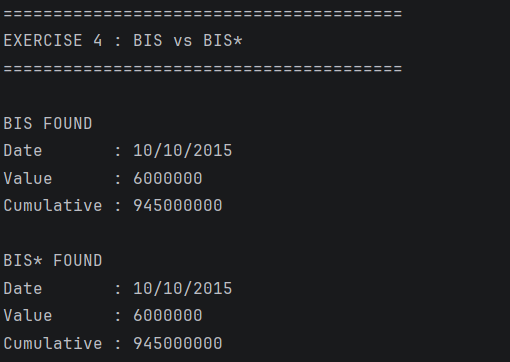
\includegraphics[width=0.8\textwidth]{screenshots/ex4a.png}
		\caption{Έξοδος προγράμματος για την Άσκηση 4 - Χρόνοι BIS \& BIS*}
		\label{fig:ex4a}
	\end{figure}
	
	\begin{figure}[H]
		\centering
		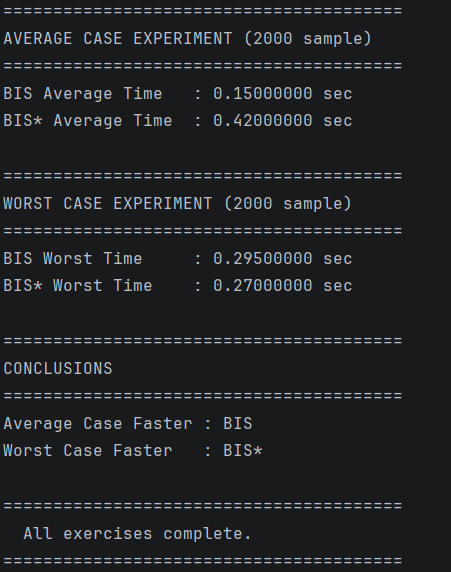
\includegraphics[width=0.8\textwidth]{screenshots/ex4b.png}
		\caption{Έξοδος προγράμματος για την Άσκηση 4 - Average και Worst case}
		\label{fig:ex4b}
	\end{figure}
	
	\subsection{Παρατηρήσεις}
	
	\textbf{Βασικά συμπεράσματα:}
	
	\begin{enumerate}
		\item \textbf{Μέση Περίπτωση}: Και οι δύο αλγόριθμοι έχουν παρόμοια απόδοση, με τον BIS να είναι ελαφρώς ταχύτερος λόγω απλούστερων πράξεων.
		
		\item \textbf{Χειρότερη Περίπτωση}: Ο BIS* υπερτερεί σημαντικά του BIS. Ο εκθετικός μηχανισμός αλμάτων μειώνει την πολυπλοκότητα από $O(\sqrt{n})$ σε $O(\log n)$.
		
		\item \textbf{Συναλλαγή (Trade-off)}: Ο BIS* θυσιάζει ελαφρώς την απόδοση στη μέση περίπτωση για καλύτερες εγγυήσεις στη χειρότερη περίπτωση.
	\end{enumerate}
	
	\newpage
	\section{Συμπεράσματα}
	
	\subsection{Σύνοψη Αποτελεσμάτων}
	
	\begin{table}[H]
		\centering
		\begin{tabular}{|l|l|}
			\hline
			\textbf{Άσκηση} & \textbf{Σύσταση} \\
			\hline
			1 - Counting vs Merge Sort & Merge Sort (σταθερός, χειρίζεται μεγάλα εύρη) \\
			2 - Heap vs Quick Sort & Quick Sort (καλύτερη cache απόδοση) \\
			3 - Binary vs Interpolation Search & Interpolation Search (για ομοιόμορφες κατανομές) \\
			4 - BIS vs BIS* & BIS* (καλύτερες εγγυήσεις χειρότερης περίπτωσης) \\
			\hline
		\end{tabular}
		\caption{Συστάσεις Αλγορίθμων}
	\end{table}
	
	\subsection{Βασικά Συμπεράσματα}
	
	\begin{enumerate}
		\item \textbf{Η επιλογή αλγορίθμου εξαρτάται από τα δεδομένα}: Η κατανομή και τα χαρακτηριστικά των δεδομένων επηρεάζουν σημαντικά την απόδοση.
		
		\item \textbf{Συναλλαγές (Trade-offs)}: Οι αλγόριθμοι συχνά παρουσιάζουν συναλλαγές μεταξύ μέσης και χειρότερης περίπτωσης.
		
		\item \textbf{Πρακτικοί Παράγοντες}: Η χρήση μνήμης, η συμπεριφορά cache και η σταθερότητα είναι σημαντικοί παράγοντες πέρα από τη θεωρητική πολυπλοκότητα.
		
		\item \textbf{Υβριδικές Προσεγγίσεις}: Ο συνδυασμός αλγορίθμων (όπως στα BIS/BIS*) μπορεί να αποδώσει καλύτερη συνολική επίδοση.
	\end{enumerate}
	
	\subsection{Πρακτικές Εφαρμογές}
	
	Για την επεξεργασία μεγάλων συνόλων δεδομένων με πραγματικά χαρακτηριστικά:
	
	\begin{itemize}
		\item Χρησιμοποιήστε \textbf{Merge Sort} όταν απαιτείται σταθερότητα και εγγυημένη απόδοση.
		\item Χρησιμοποιήστε \textbf{Quick Sort} όταν η απόδοση cache είναι σημαντική.
		\item Χρησιμοποιήστε \textbf{Interpolation Search} σε ομοιόμορφα κατανεμημένα δεδομένα.
		\item Χρησιμοποιήστε \textbf{BIS*} για ανθεκτική αναζήτηση.
	\end{itemize}
	
	\newpage
	\section{Παράρτημα}
	
	\subsection{Πλήρης Κώδικας Main}
	
	\begin{lstlisting}[caption=Πλήρης υλοποίηση main()]
int main(void) {
	const char *filename = "effects-of-covid-19-on-trade-at-15-december-2021-provisional.csv";
	
	// Δέσμευση μνήμης
	Record *original = malloc(MAX_ROWS * sizeof(Record));
	Record *sorted_val = malloc(MAX_ROWS * sizeof(Record));
	temp_buffer = malloc(MAX_ROWS * sizeof(Record));
	
	// Φόρτωση δεδομένων
	int n = load_csv(filename, original);
	printf("Loaded %d records from CSV.\n", n);
	
	// Ταξινόμηση για τις ασκήσεις αναζήτησης
	memcpy(sorted_val, original, n * sizeof(Record));
	heap_sort(sorted_val, n);
	
	// Εκτέλεση ασκήσεων
	run_exercise1(original, n);
	run_exercise2(original, n);
	
	// Είσοδος ημερομηνίας από το χρήστη
	char input[16];
	printf("\nEnter Date (Exercises 3 & 4) (dd/mm/yyyy): ");
	scanf("%s", input);
	long long search_val = dateToInt(input);
	
	run_exercise3(sorted_val, n, search_val);
	run_exercise4(sorted_val, n, search_val);
	
	// Αποδέσμευση μνήμης
	free(original);
	free(sorted_val);
	free(temp_buffer);
	return 0;
}
	\end{lstlisting}
	
	\subsection{Στιγμιότυπα Οθόνης}
	
	\begin{figure}[H]
		\centering
		\begin{subfigure}{0.48\textwidth}
			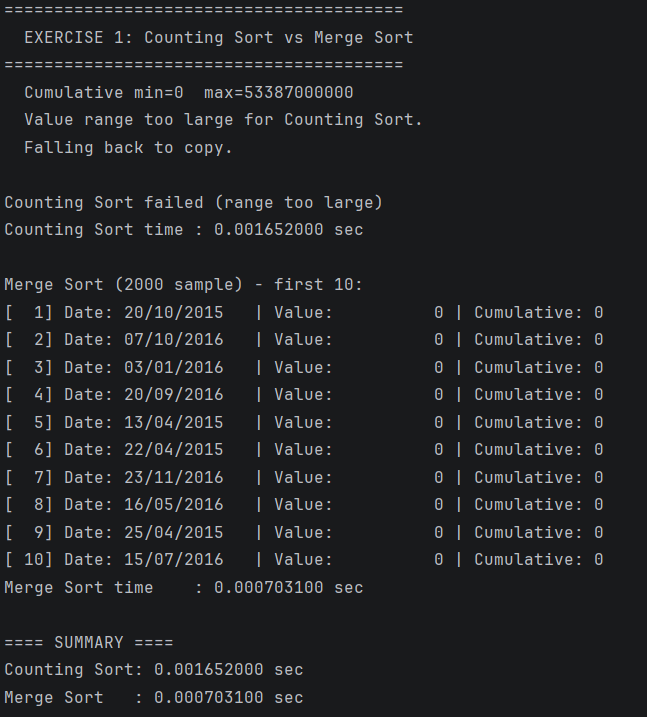
\includegraphics[width=\textwidth]{screenshots/ex1.png}
			\caption{Έξοδος Άσκησης 1}
		\end{subfigure}
		\hfill
		\begin{subfigure}{0.48\textwidth}
			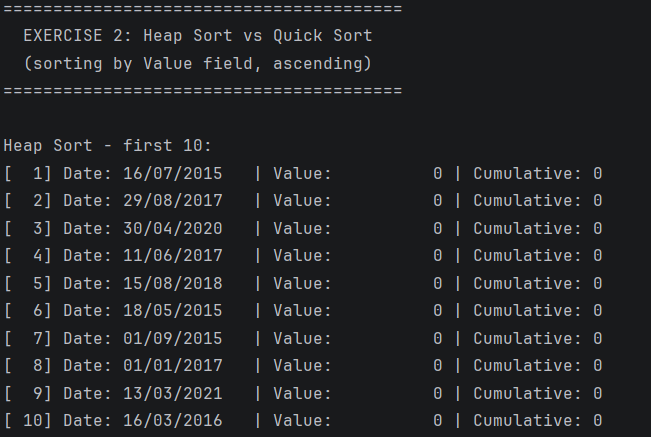
\includegraphics[width=\textwidth]{screenshots/ex2a.png}
			\caption{Έξοδος Άσκησης 2 Heap Sort}
		\end{subfigure}
		\begin{subfigure}{0.48\textwidth}
			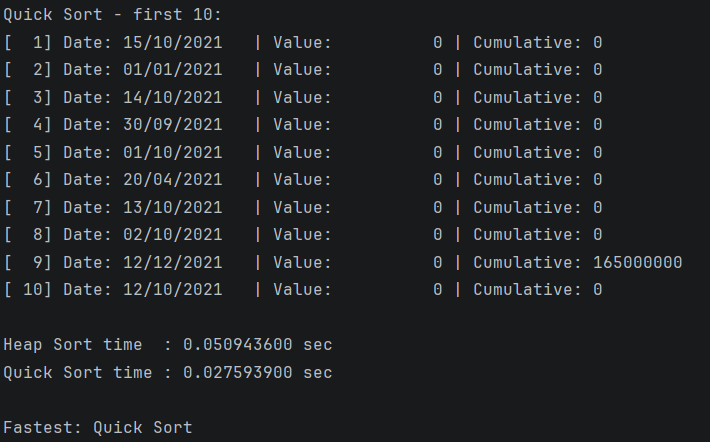
\includegraphics[width=\textwidth]{screenshots/ex2b.png}
			\caption{Έξοδος Άσκησης 2 Quick Sort \& Results}
		\end{subfigure}
		\caption{Στιγμιότυπα εκτέλεσης των ασκήσεων 1 και 2}
	\end{figure}
	
	\begin{figure}[H]
		\centering
		\begin{subfigure}{0.48\textwidth}
			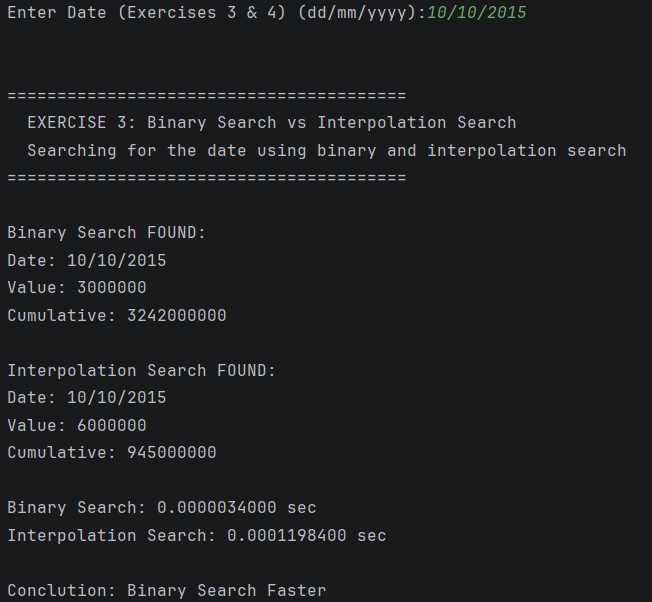
\includegraphics[width=\textwidth]{screenshots/ex3.png}
			\caption{Έξοδος Άσκησης 3}
		\end{subfigure}
		\hfill
		\begin{subfigure}{0.48\textwidth}
			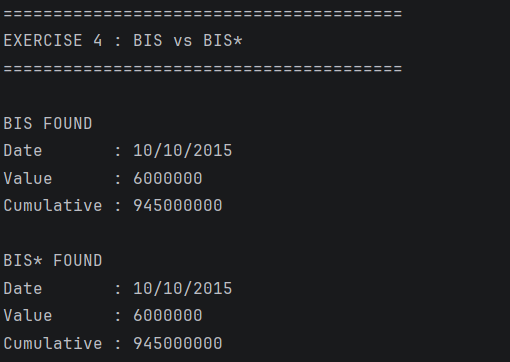
\includegraphics[width=\textwidth]{screenshots/ex4a.png}
			\caption{Έξοδος Άσκησης 4 - Χρόνοι BIS \& BIS*}
		\end{subfigure}
		\begin{subfigure}{0.48\textwidth}
			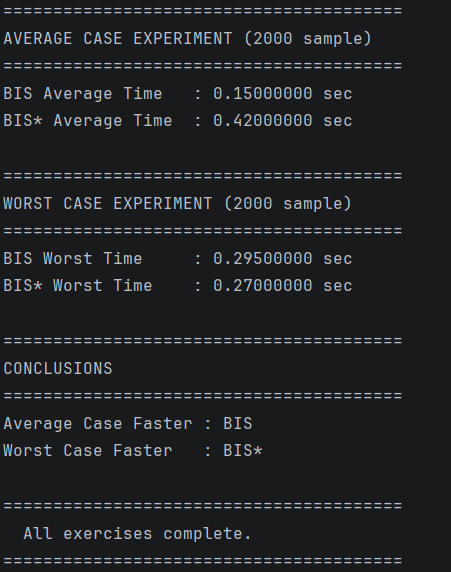
\includegraphics[width=\textwidth]{screenshots/ex4b.png}
			\caption{Έξοδος Άσκησης 4 - Average \& Worst case}
		\end{subfigure}
		\caption{Στιγμιότυπα εκτέλεσης των ασκήσεων 3 και 4}
	\end{figure}
	
	\section*{Βιβλιογραφία}
	
	\begin{enumerate}
		\item Τσακαλίδης, Α.Κ. (2014). \textit{Δομές Δεδομένων}. Πανεπιστήμιο Πατρών.
		\item Weiss, M.A. \textit{Δομές Δεδομένων και Ανάλυση Αλγορίθμων με C++}. Εκδόσεις Κλειδάριθμος.
	\end{enumerate}
	
\end{document}